\section{Introduction}
\begin{frame}
  \frametitle{Background and Motivation}

FPGAs are making their way into data centers to boost the computing power
	and the overall power efficiency.


\begin{columns}

\begin{column}{0.2\textwidth}
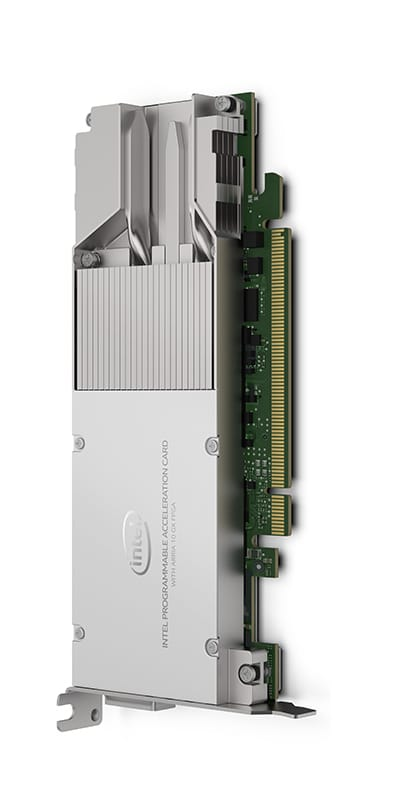
\includegraphics[scale=0.2]{./background/intel_fpga_nic.jpg}
\end{column}

\begin{column}{0.8\textwidth}
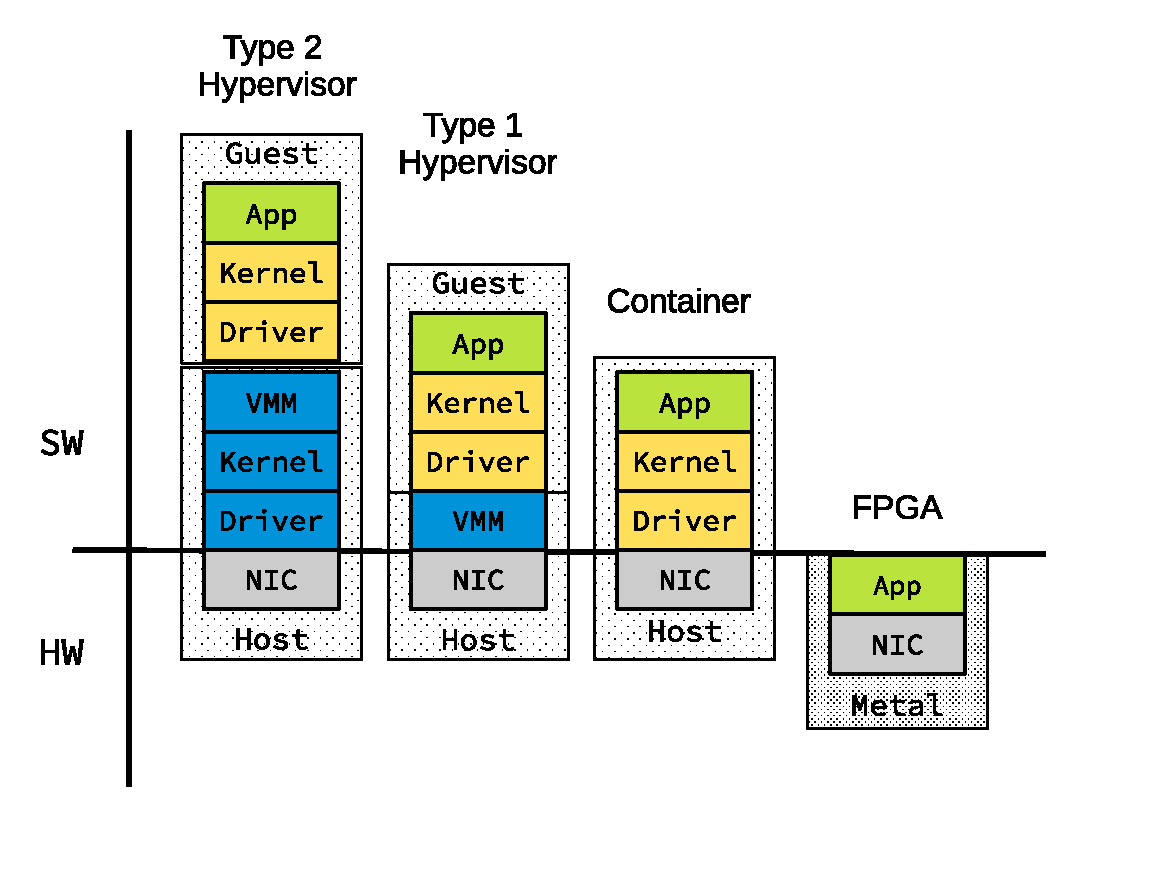
\includegraphics[scale=0.5]{./background/server_configuration.eps}
\end{column}


\end{columns}

\end{frame}




\note{Applikationer og Big-Data udregninger flytter til Cloud, drevet af store
data centre.\\

Disse data-centre kraever rigtigt meget plads, store maengder af stroem og er i stigende grad svaere
at vedligeholde og udvide.\\

De fleste data-centre er derfor begyndt at aflaste beregningerne til FPGAer,
som fjerner meget af overhead til beregningerne\\

FPGA bruges til at få en computer til at køre hurtigere hvis de mest brugte
instruktioner, skrives direkte ned i hardwaren\\

PROBLEMET er at der kun kan vaere en begreanset antal af FPGAer i konventionele
servere

}



% Talking points:


% > In the current era of big data, computationally heavy applications are
% moving to the cloud. ... Consuming wast amount of energy and are increasingly
% complex to maintain and improve

% > To combat this, DC servers offload the computation onto FPGAs

% <SHOW GRAPH HERE>

% > However, this is not scalable in the conventional DC architecture, as the
% FPGAs are directly connected to CPUs using a PCI bus.

% <SHOW CONVENTIONAL DC>

% > Disaggregated DC architecture proposes FPGA be turned into a
% self-contained standalone appliance capable of managing itself. Then, it is
% connected to the rest of the Data-Center by a local network. This enables the
% DC to pack even more computing capacity into the same physical volume at the
% same, or even lower, energy consumption.

% <SHOW DISAGGREGATED DC>

% > This can increase the density of the servers by sharing resources
% such as power supplies, cooling, fans, networking uplinks, and other management
% infrastructures.

% > In this thesis, we want to make a self-contained TCP/IP stack on an FPGA
% using SME.



\begin{frame}

A conventional data center architecture
\begin{figure}
	\centering
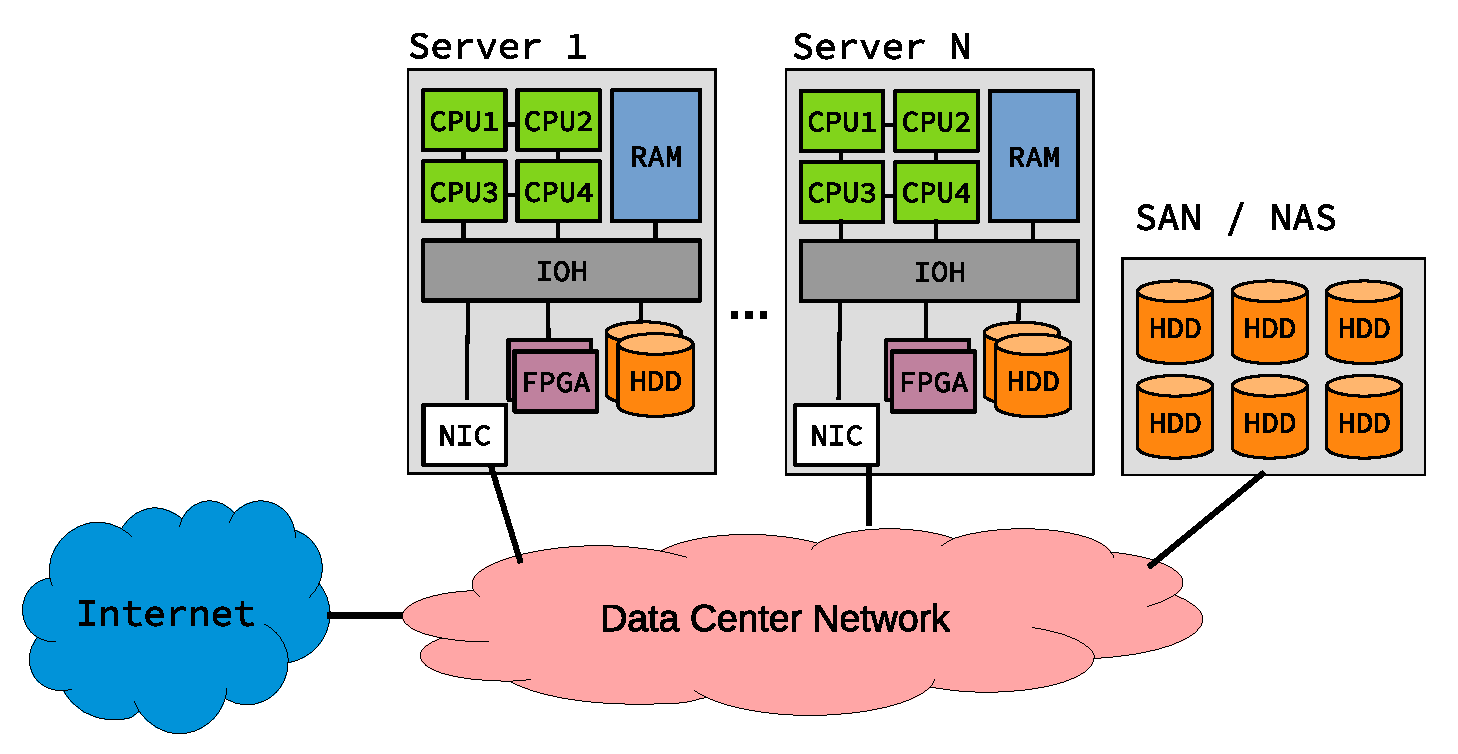
\includegraphics[scale=0.5]{./background/dc_architectures_conventional.eps}

\end{figure}

\end{frame}


\begin{frame}
	Proposed disaggregated data center architecture (\cite{7830659})
\begin{figure}
	\centering
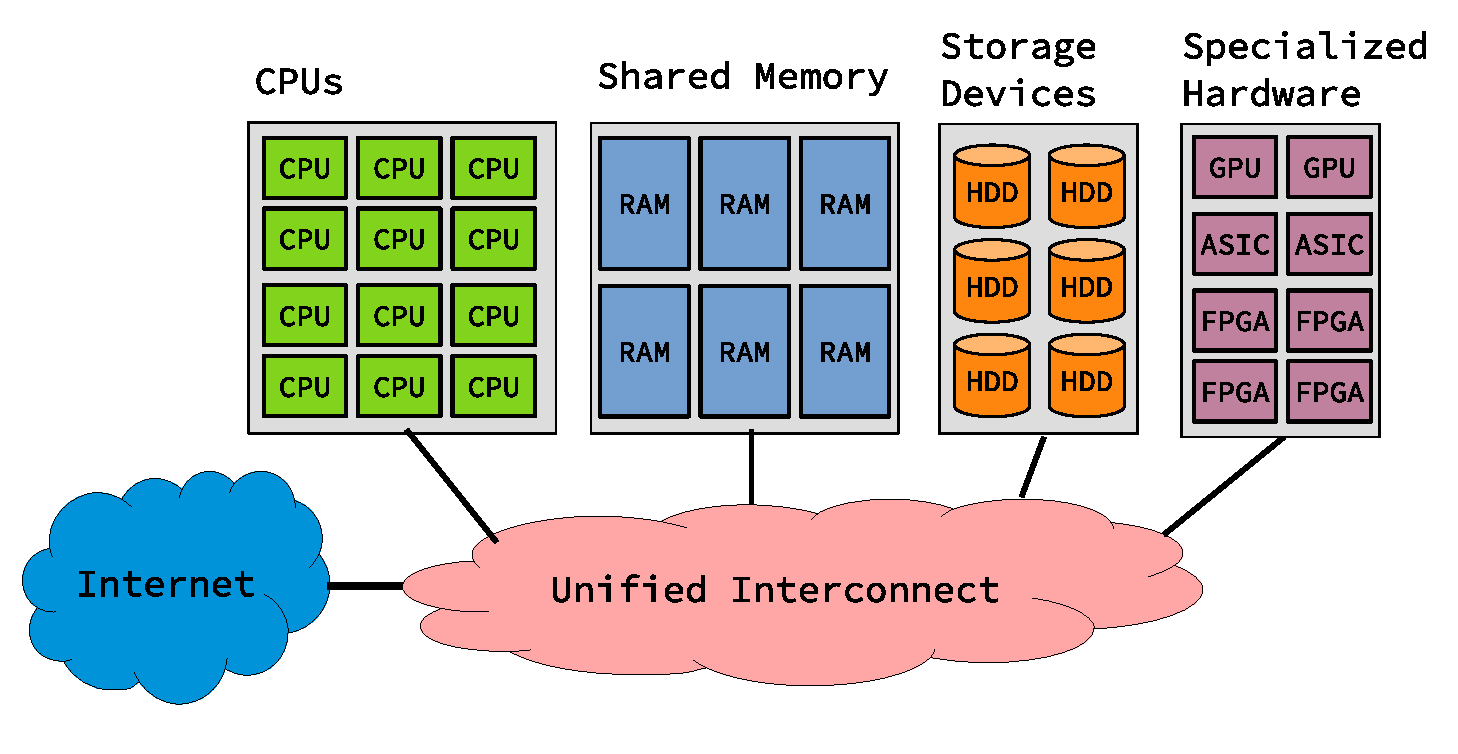
\includegraphics[scale=0.5]{./background/dc_architectures_disaggregated.eps}
\end{figure}
\end{frame}

\note{Hvis man splitter resourcerne op, kan man takket været FPGA få bedre
ydeevne på det samme areal, samt nemmere håndtering af servere og deres komponenter. }

\begin{frame}
FPGA usage
\begin{figure}
	\centering
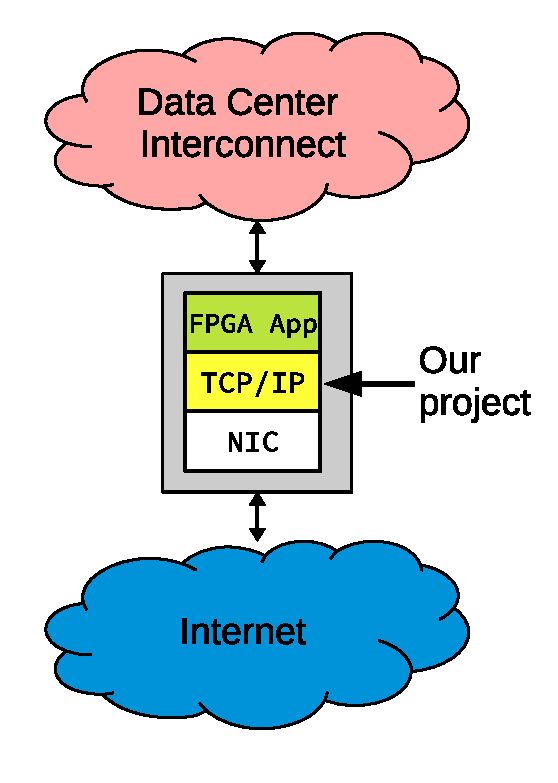
\includegraphics[scale=0.5]{./background/fpga_usage.eps}
\end{figure}

\end{frame}

\begin{frame}
The Internet

\begin{figure}
	\centering
\includegraphics[scale=0.15]{./background/internet_map.jpg}
\label{fig: Internet map}
\caption{Map of about 30\% of the accessible the endpoints on the Internet}
\end{figure}

\end{frame}


\begin{frame}
The Internet Protocol Suite -- A scenario
\begin{figure}
	\centering
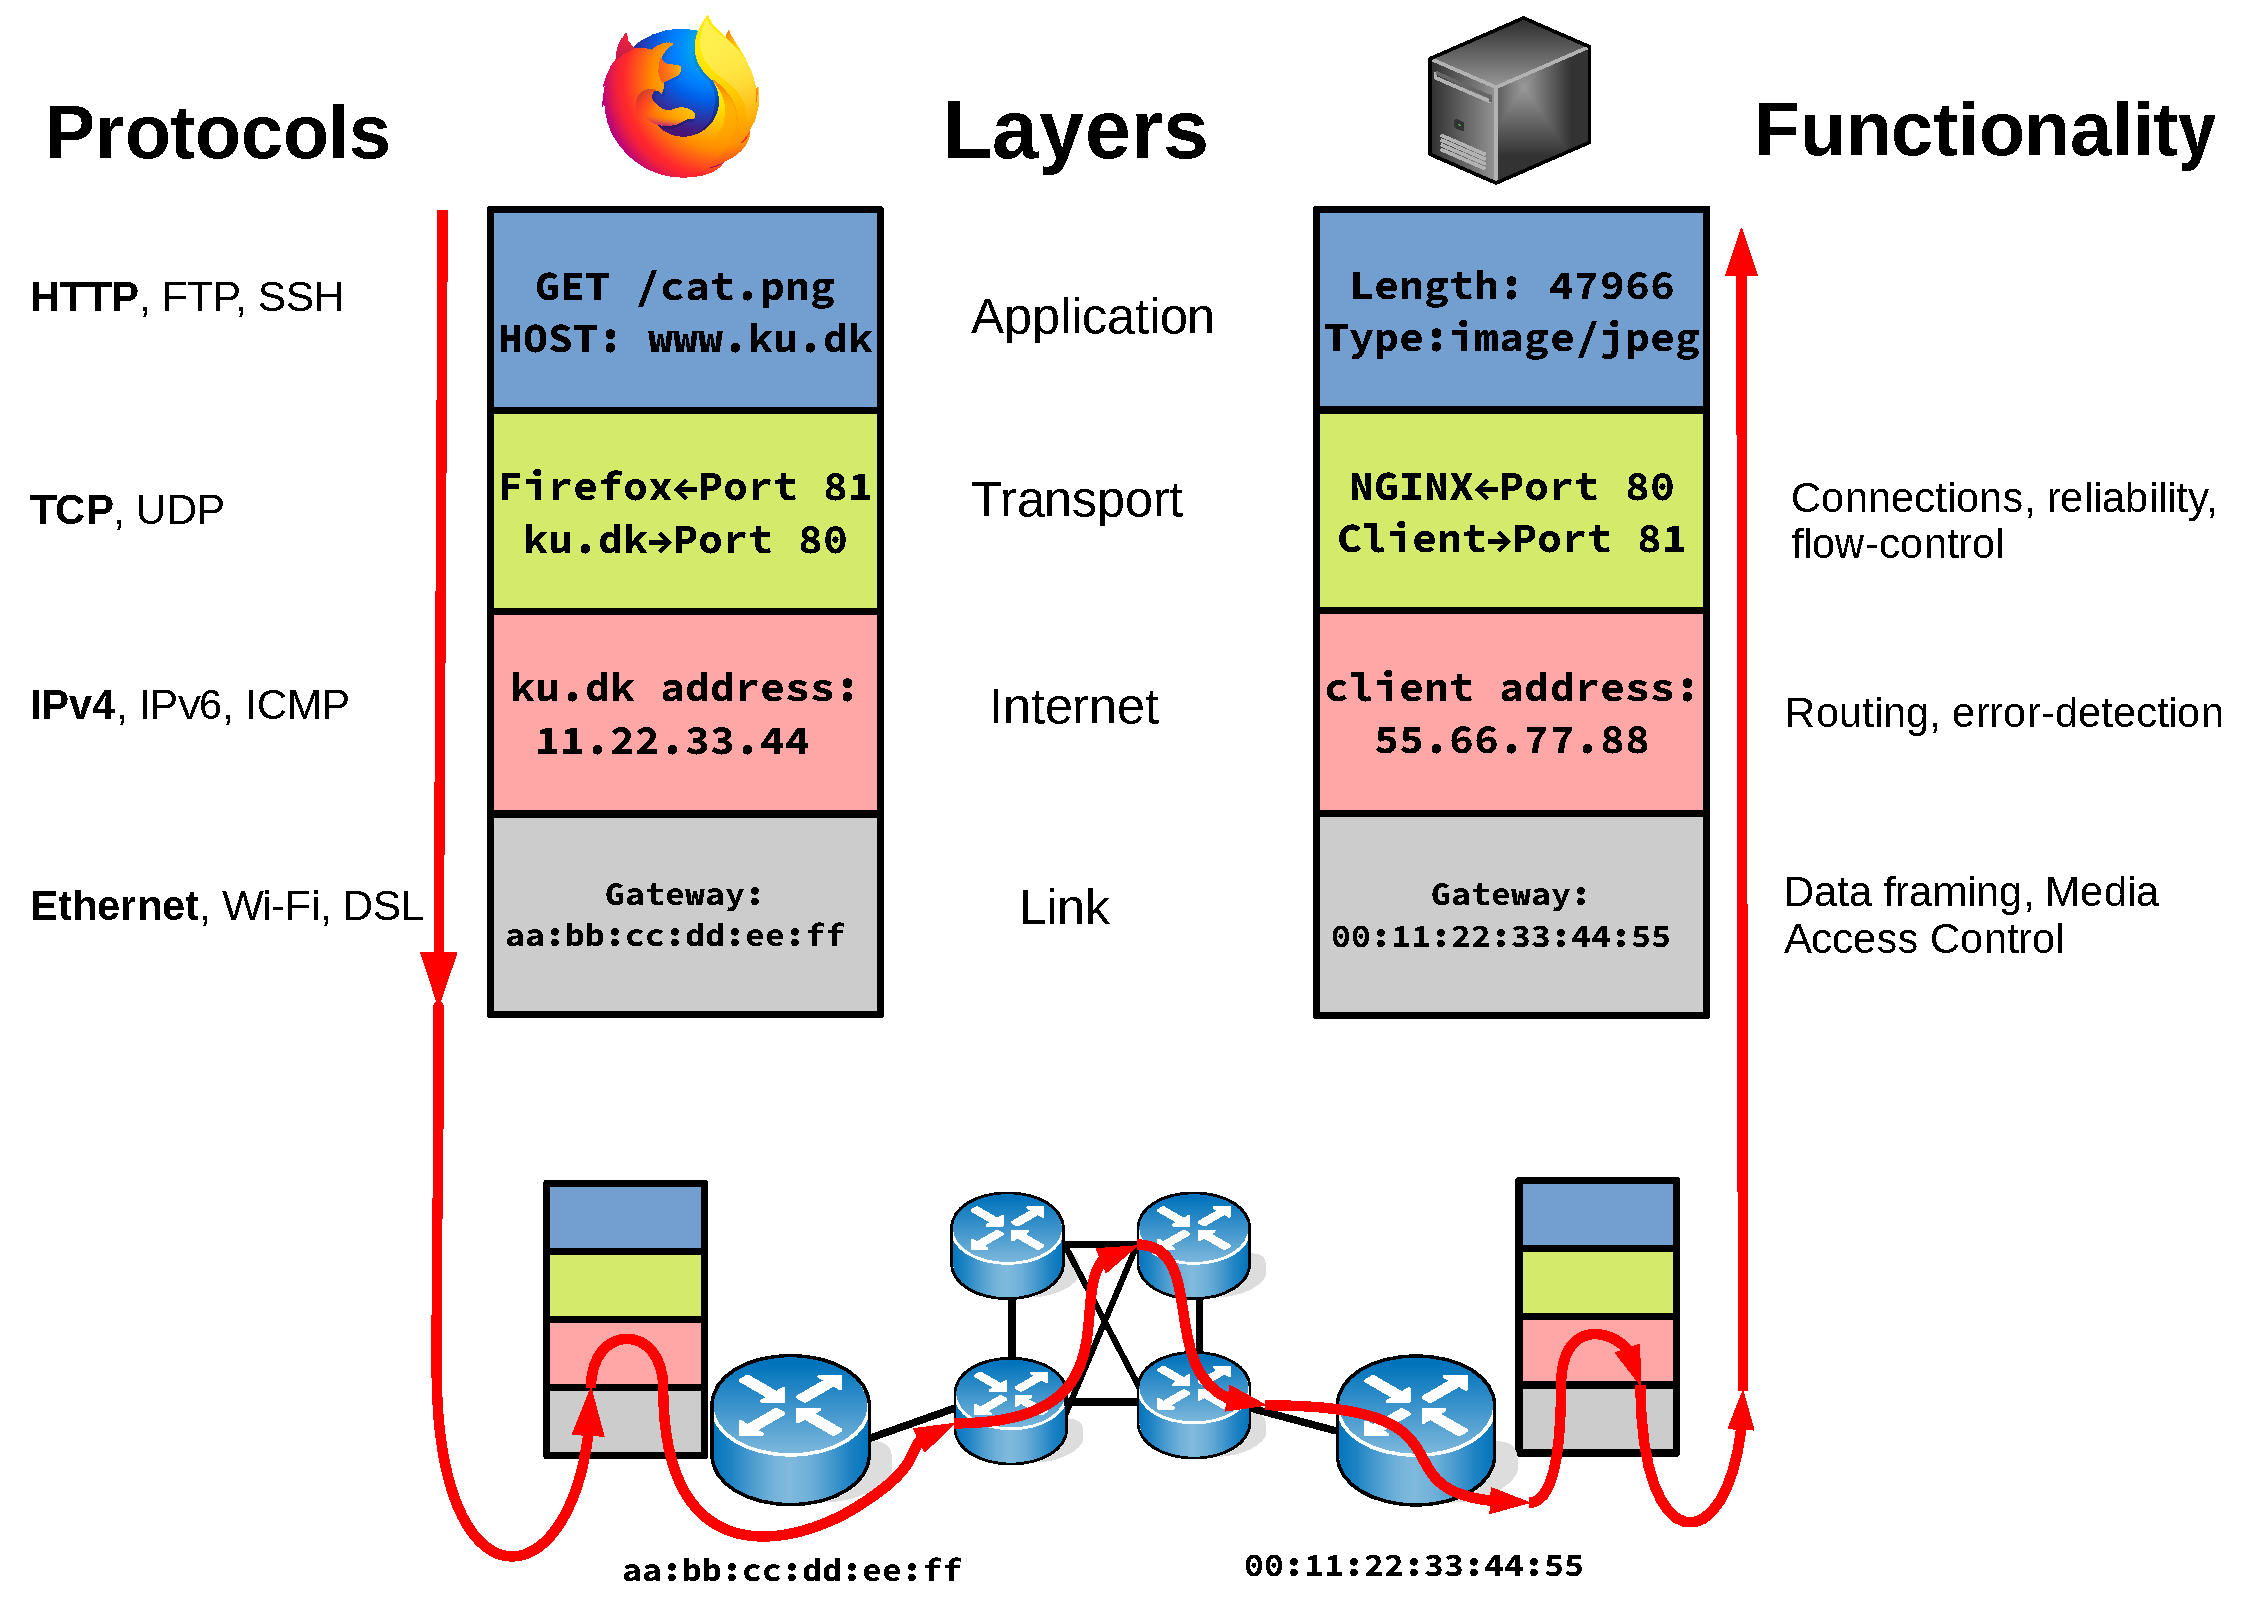
\includegraphics[scale=0.28]{./background/internet_scenario.pdf}
\end{figure}



\end{frame}


\begin{frame}
Design with the 4 layers in mind
\begin{figure}
	\centering
%\includegraphics[scale=0.5]{./background/frame.eps}
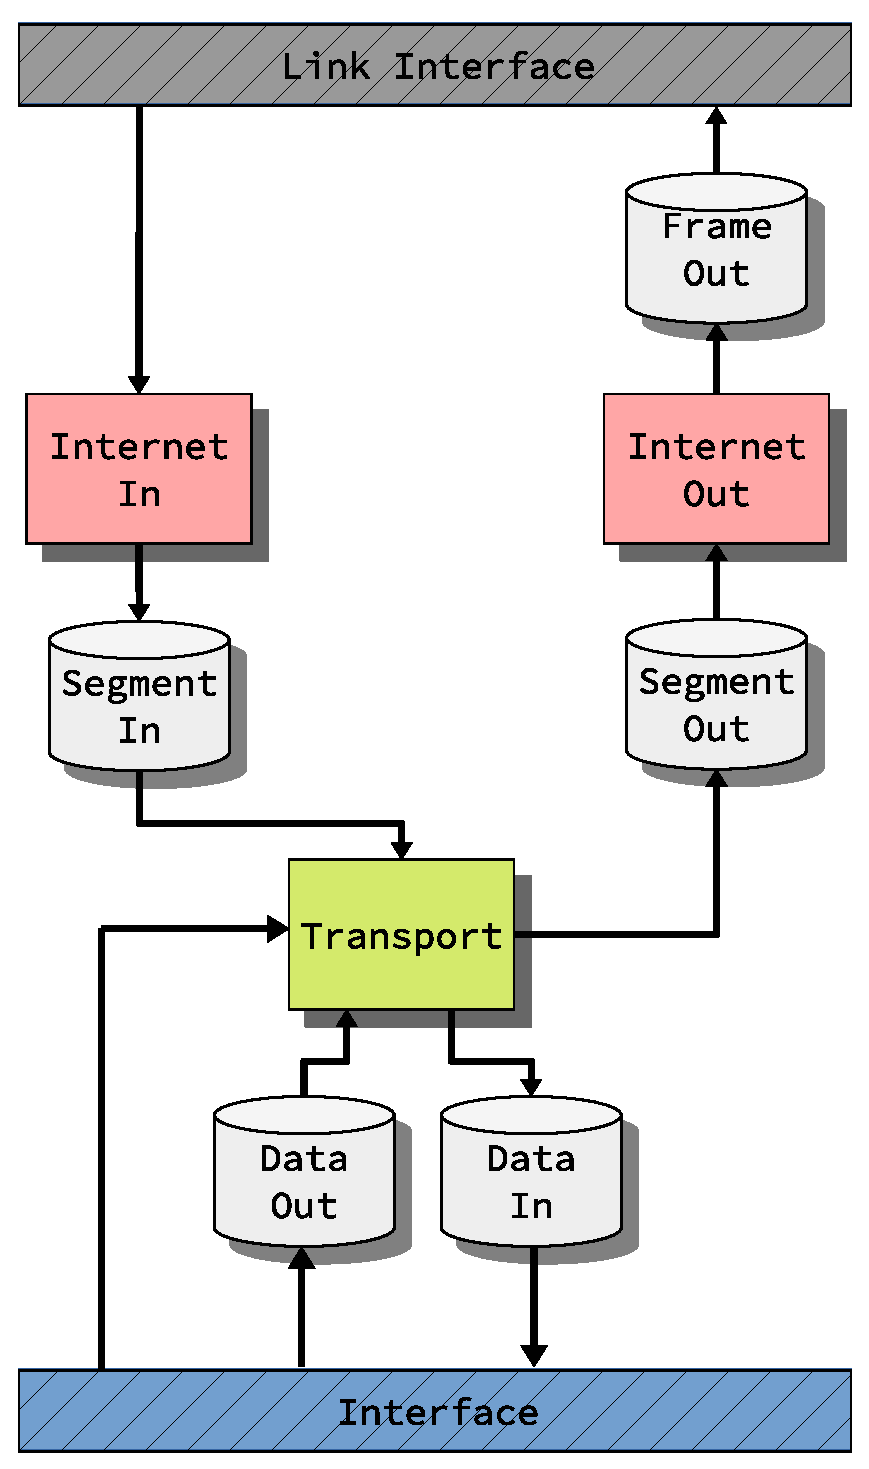
\includegraphics[scale=0.3]{./background/design_2.eps}
\end{figure}
\end{frame}



% - Network Stack Specialization for Performance\\
% - Disaggregated FPGAs\\
% - A Cloud-Scale Acceleration Architecture

% Talking points:
% 1. In the current era of big data, computationally heavy applications are
% moving to the cloud.

% 2. DC infrastructures are being redesigned to pack ever more compute capacity
% into the same volume and power envelops

% 3. This is done by increasing the density of the servers by sharing resources,
% such as power supplies, cooling, fans, networking uplinks, and other management
% infrastructures.

% 4. Problem -- currently, FPGAs are connected directly to CPUs using some PCI
% bus, making the separation hard. [0] proposes FPGA must be turned into a
% self-contained standalone appliance capable of managing itself. Then, it is
% connected to the rest of the Data-Center by a local network.

% 5. In this thesis, we want to make a self-contained TCP/IP stack on an FPGA
% using SME.


% [0]: [Disaggregated FPGAs]


